\clearpage
\section{Laser} %ROHS complian and Class 1 laser - removing the casing can cause problems and decalssify it

Our laser of choice, the LIDAR-Lite SEN-13167, is a SoC (System-on-a-Chip) solution for optical distance measurements applications. It has a 4.7 - 5.5 V nominal and 6 V potentially maximum DC operating range. The sensor has a theoretical limit of 40m range and 100Hz rep rate. The laser emitters' accuracy is estimated to be +/- 2.5cm with an aquisition time of less then 0.02sec. These specifications allows us to get an accurate image of the environments specified in our test cases~\cite{lidarsum}.

\begin{figure}[H]
	\centering
	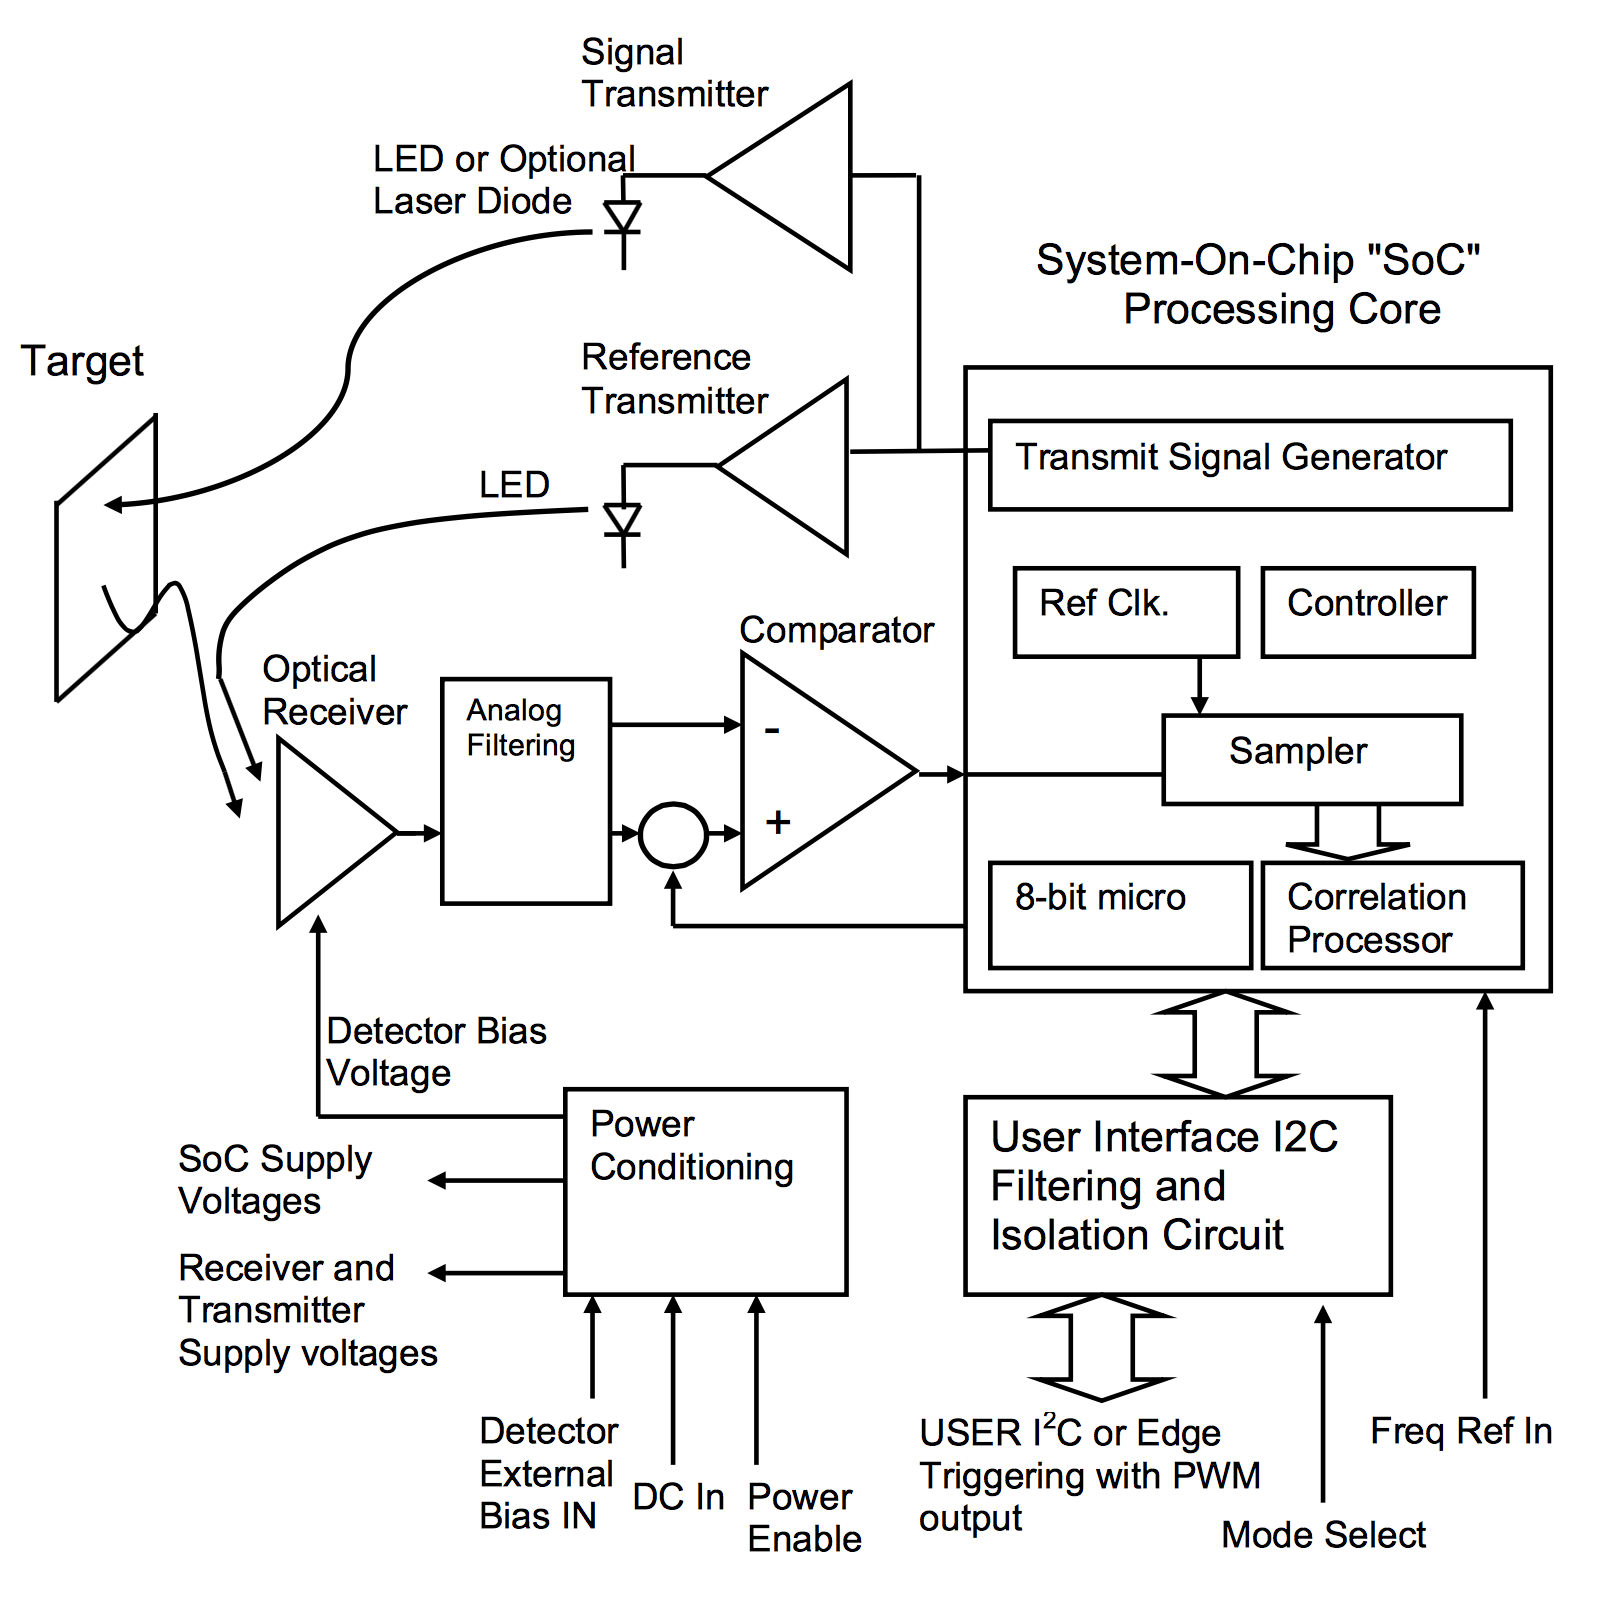
\includegraphics[scale=.4]{images/internallidar.png}
	\caption{An overview of the laser's internals}
	\label{fig:internallidar}
\end{figure}

As we discussed prior how rangefinders lasers work (Figure~\ref{fig:rangefinderIMG}), our laser has two 14mm optic lenses, one as a transmitter emitting a 905nm infrared pulse and a receiver, measuring the time it takes for the pulse to travel back and the angle it comes in.

At distances less than a meter, the pulse is about the size of the receiver optic lens, at distances longer than that, you can estimate it using the following equation: \textit{d/100 = psize}, where d = distance and psize = the pulse size at that specific distance, in the units they are measured in. The actual spread is $\sim 8$ Mil or $\sim1/2$ degree\cite{spreadofbeam}.

It is possible to receive multiple valid return signals from a single measurement if the pulse illuminates more than one surface along the beam path. The sensor has the capability to process two distinct reflections as long as they are separated by more than 3.5 meters and the reflection at the shorter distance does not saturate the correlation record masking the more distant object. 

The figure below shows an example of two reflections in the signal correlation record separated by approximately 3.5 meters.

\begin{figure}[H]
	\centering
	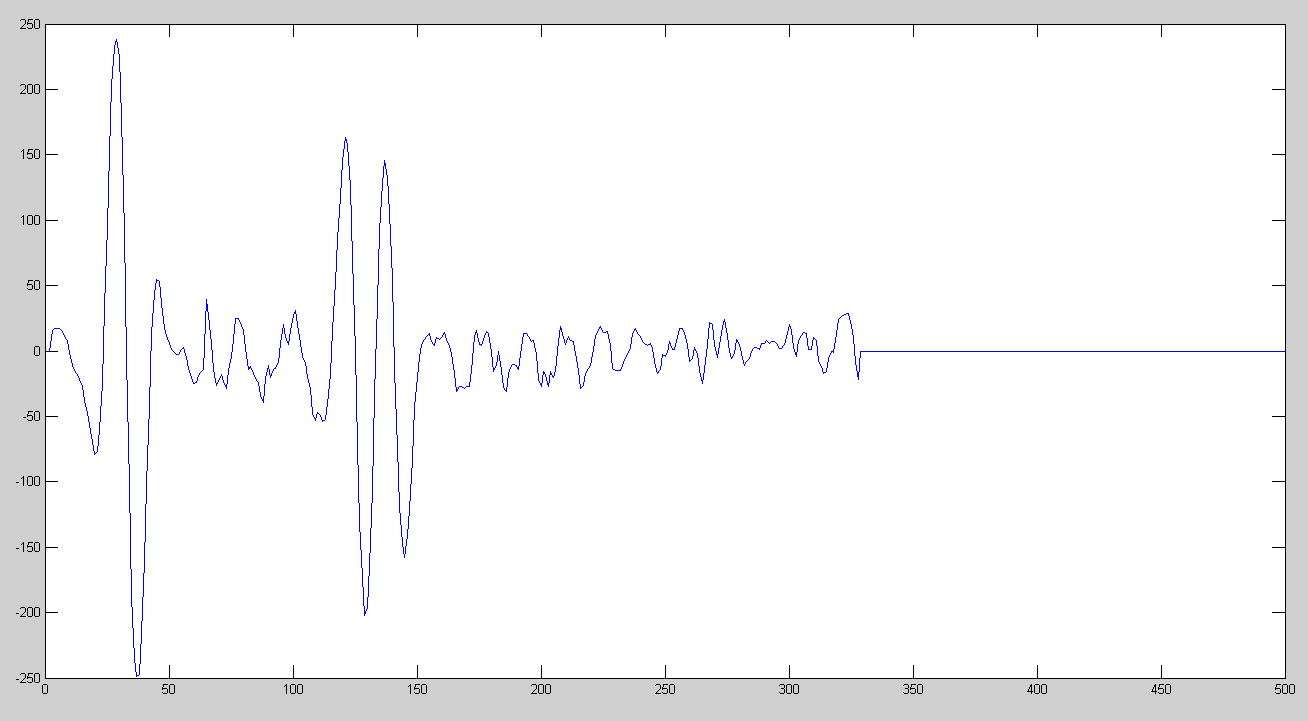
\includegraphics[scale=.2]{images/tworeflection.png}
	\caption{Measuring two valid return signals from one measurement~\cite{howtopulse}}
	\label{fig:tworeflections}
\end{figure}

The sensor detection criteria may be selected to pick the nearer signal, the more distant signal or the strongest signal strength.

A reference signal fed from the transmitter prior to the distance measurement and a received pulse reflected from the target. The time delay between these two stored signals is estimated through a signal processing approach known as \textit{correlation}, which effectively provides a signature match between these two closely related signals. This accurately calculates the time delay, which is translated into distance based on the known speed-of-light~\cite{howtopulse}.

By default the sensor runs about 50 Hz (could vary given the signal strength and distance). To optimize the rep rate, it is possible to decrease the max-acquisition count (on register 0x02). By default register 0x02 is 0x80, if you decrease this the maximum number of acquisitions the sensor can take and use to get a reading will decrease\cite{reprate}.

\pagebreak
The assembling of the laser happened in the following way:

\begin{figure}[H]
	\centering
	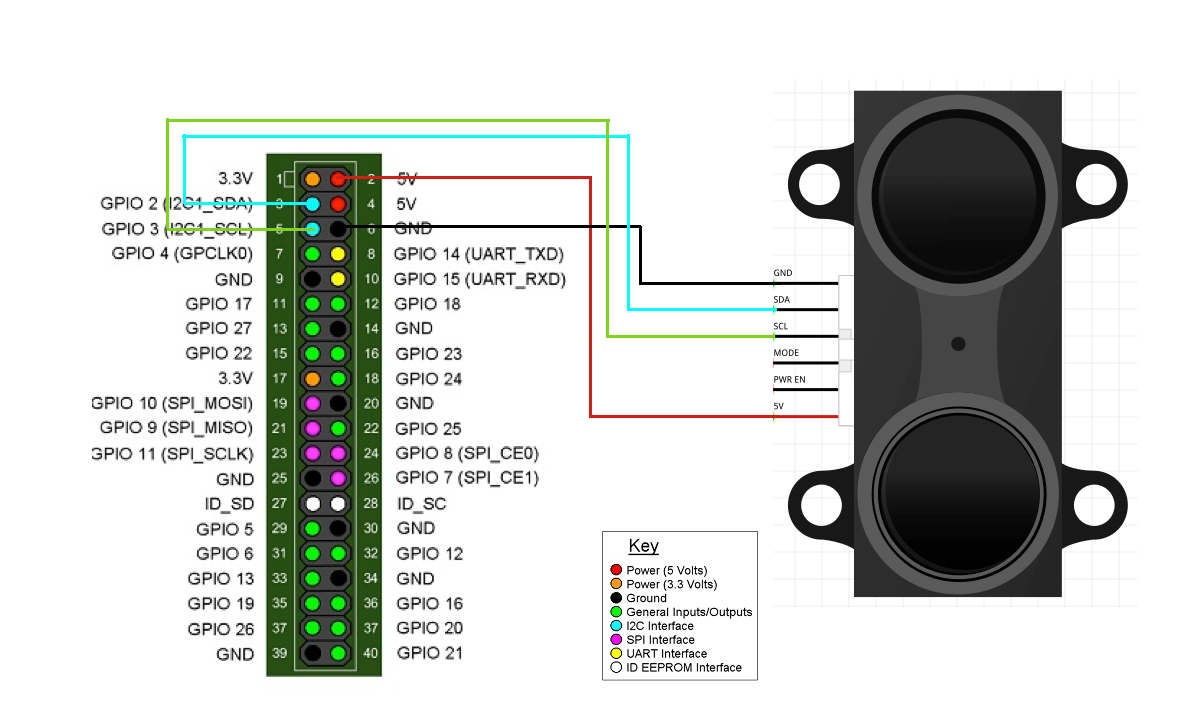
\includegraphics[scale=.3]{images/laderraspberryconnection.png}
	\caption{The pinout and wiring of the LIDAR and Raspberry Pi}
	\label{fig:wiringlidarpi}
\end{figure}

\begin{table}[H]
	\centering
	\begin{tabular}{|l|l|l|}
		\hline
		\textbf{Raspberry pin} & \textbf{Description} & \textbf{LIDAR pin} \\ \hline
		2 & 5V & Red \\ \hline
		5 & GND & Black \\ \hline
		4 & SCL & Green \\ \hline
		3 & SDA & Blue \\ \hline
	\end{tabular}
	\caption{The pins of the microcontroller mapped to the laser pins}
\end{table}

The laser can be interfaced through I2C or PWM~\cite{lidarsum}. The default I2C address for the laser is 0x62, which we could validate by running:
\lstset{language=sh}
\begin{lstlisting}
	>>	sudo i2cdetect -y 1
	>>
		  0  1  2  3  4  5  6  7  8  9  a  b  c  d  e  f
		  00:          -- -- -- -- -- -- -- -- -- -- -- -- --
		  10: -- -- -- -- -- -- -- -- -- -- -- -- -- -- -- --
		  20: -- -- -- -- -- -- -- -- -- -- -- -- -- -- -- --
		  30: -- -- -- -- -- -- -- -- -- -- -- -- -- -- -- --
		  40: -- -- -- -- -- -- -- -- -- -- -- -- -- -- -- --
		  50: -- -- -- -- -- -- -- -- -- -- -- -- -- -- -- --
		  60: -- -- 62 -- -- -- -- -- -- -- -- -- -- -- -- --
		  70: -- -- -- -- -- -- -- -- 
\end{lstlisting}

We started using a library called lidarLite, which provides a simple C interface to the LIDAR on a Raspberry. It is based on the WiringPi interface, which is a GPIO access library written in C for the BCM2835 SoC used in the Raspberry Pi. It is usable from C and C++ and many other languages with suitable wrappers. It was designed very familiarly to Arduino's wiring library.

With the lidarLite library, we managed to set up a connection using the I2C protocol. By enabling the built in I2C support in the Raspberry Pi kernel, and after the wiring of the components, a connection has been set up between the LIDAR laser and the controller.



%https://learn.adafruit.com/adafruits-raspberry-pi-lesson-4-gpio-setup/configuring-i2c
%https://github.com/answer17/lidarLite

A small program was written in order to test the output of the laser sensor, namely to read out the distance value of the next closest point in centimeters. 

% sample output here

This output is generated by the function called \textit{lidar\_read(int fd)} from the lidarLite library. This code simply calculates the low and high value from the sensor and returns the distance measurements in centimeters, in form of an integer value. The guide on how to compile and run this small test application is available in the Appendix \\ 
%TODO: Add readme.md from laser-module folder to appendix.

%TODO: add this too in {http://wiki.ros.org/rospy/Overview/Publishers%20and%20Subscribers#Choosing_a_good_queue_size}
\lstinputlisting[firstline=47, lastline=64, title=lidarLite.c, language=C]{../code/laser_scan_publisher_tutorial/src/lidarLite.c}

We then tried to incorporate this code with a stepper-motor, so that it would return the distances around a circle.

The first version had the stepper-motor spinning the laser around at a constant speed, driven by an arduino(reference to code here), while the laser made measurements, driven by the Pi.

In order to determine how long it takes for the lidarLite lidar\_read function to execute, some testing was made

%asd.cpp

This code was run with the settings of 1000 and 2000, each version was run 3 times.

%TODO: format data nicely
Measurements of how long it takes to run lidar\_read
1000: 24.372s,24.476s,24.490s;avg:24.446s
2000: 48.400s,48.111s,48.172s;avg:48.228s

According to this data we can isolate the time it takes to execute the lidar\_read function from everything else:

$t_{total} = n*t_{lidar} + t_{rest}$

$24.446s = 1000*t_{lidar} + t_{rest}$
$48.228s = 2000*t_{lidar} + t_{rest}$
Subtract the two equations
$23.782s = 1000*t_{lidar}$
$t_{lidar} = 0.023782s \approx 0.024s$


This proved ineffective, since the rotation and measurements were independent of eachother, which caused the measurements to be skewed over time.

Then we attempted to controll the stepper-motor with the Pi, in the same code as we were running the laser. However, the wiringPi library required root privileges, and ROS cannot be run with root privileges easily. The solution was to use a system call library to call some external code which would drive the stepper-motor. This makes the stepping and measuring synchronous, but making system call is very expensive, meaning the code is significantly slower that the top speed of the laser.

\lstinputlisting[firstline=55, lastline=109, title=mainCode.cpp, language=C++]{../code/laser_scan_publisher_tutorial/src/laser_scan_publisher.cpp}

\lstinputlisting[firstline=1, lastline=16, title=gpioWrapper, language=sh]{../code/gpioThing.sh}
The only purpose of this code is to be called from the main file. The gpio utility is capable of interfacing with the GPIO pins on the Pi without root privileges. The change from low to high causes a micro-step, and 8 micro-steps make one full step.
